In order to increase the speed of our program, it has been decided to parallelize it on a set of clusters of multi-core machines, in the more complex possibilty. But there are many ways to parallelize our algorithm and we have to choose how we want to do it. In a first time, let's talk about the parallelization method which has the most potential, then, we will see which of them can be suitable for our cases.
\subsubsection{Previous Work}
In the last report, we talked about the different methods, their advantages and their drawbacks. There are mainly two parallelization methods that are efficient in the conditions of our project, in terms of speed.

The first one is called the Root Parallelization. It consists in giving the tree to develop to every thread, let them develop it randomly without any communication with the environment
during a certain amount of time and then, merge the results of each tree.
This method has the great benefit of minimizing the communication between the actors (in this case, the threads).
They only communicate at the beginning and at the end of the algorithm, without needing any further synchronization. The Root Parallelization is depicted in figure \ref{fig:root}.

\begin{figure}[!ht] 
\centerline{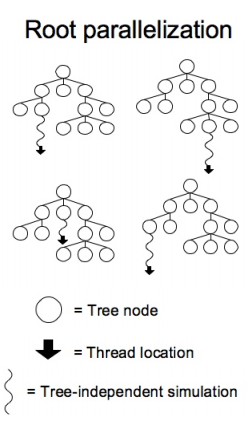
\includegraphics[scale=0.60]{3Methods/3.1Parallelization_Method/root.png}}
   \caption{Overview of Root Parallelization \cite{parallel_comp}}
\label{fig:root}
\end{figure}

The other efficient parallelization method is called UCT-Treesplit and is depicted if figure \ref{fig:treesplit}. It looks like Root Parallelization as it gives to each actor the same tree to develop.
But contrary to Root Parallelization, when the tree is developed on a certain node, it goes on working packages \footnote{A working package is a set of nodes that can be possibly developped.} who are distributed among every actor. The repartition of the packages are made by a scheduler.
In terms of performance, this method is very efficient but needs an High-Performance Computer to be optimized, or \emph{HPC}, and is very sensitive to network latency.

\begin{figure}[!ht] 
\centerline{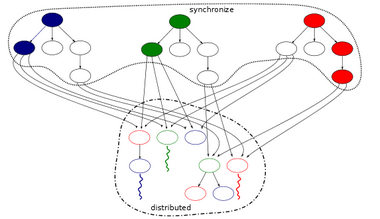
\includegraphics[scale=0.80]{3Methods/3.1Parallelization_Method/treesplit.png}}
   \caption{Overview of UCT-Treesplit Algorithm \cite{treesplit}}
\label{fig:treesplit}
\end{figure}


We have to choose two parallelization methods, one for the cluster parallelizsm and another for the shared memory parallelism.
\subsubsection{Cluster Parallelism}
For the cluster parallelism, we have to take into account the fact that communication will be done by sending messages, that are relatively costly in terms of performance.
Moreover, as the network can have latency, it is best to minimize the communication between the computers and that's why Root Parallelization has been chosen over 	UCT-Treesplit.
Root Parallelization reduces the cost in communication at maximum, is very simple to implement, does not depend on the configuration of each computer and is very efficient\cite{parallel_comp}.

\subsubsection{Shared Memory Parallelism}
For the shared memmory parallelism, we can choose between many methods but, as seen previously, Root Parallelisation is the better one.\cite{parallel_comp}
That is why this method will also be chosen for the shared memory parallelism. This way, the global strategy of our program will be simple, efficient and homogeneous.